\documentclass[a4paper,12pt]{extarticle}
\usepackage[table,xcdraw]{xcolor}
\usepackage{pgfplots}
\usepackage[unicode, pdftex]{hyperref}
\usepackage[T2A]{fontenc}
\usepackage[utf8]{inputenc}
\usepackage[english,russian]{babel}
\usepackage{amsmath,amsfonts,amsthm, mathtools}
\usepackage{amssymb}
\usepackage{dsfont}
\usepackage{graphicx}
\graphicspath{{images/}}
\usepackage{wrapfig}
\usepackage{floatrow}
\usepackage{setspace}
\usepackage[headings]{fancyhdr}
\usepackage[margin=10pt,font={small,stretch=0,9},labelfont=bf,labelsep=period,
justification=centerlast]{caption}
\usepackage{array,tabularx,tabulary,booktabs}
\RequirePackage{multirow}
\RequirePackage{multicol}
\RequirePackage{longtable}
\usepackage{indentfirst}
\usepackage{hyperref}
\usepackage{icomma}
\newcommand*{\hm}[1]{#1\nobreak\discretionary{}
	{\hbox{$\mathsurround=0pt #1$}}{}}
\usepackage{soulutf8} 
\usepackage{etoolbox} 
\usepackage{geometry}
\geometry{top=20mm}
\geometry{bottom=20mm}
\geometry{left=20mm}
\geometry{right=20mm}
\DeclareMathOperator{\sgn}{\mathop{sgn}}
\usepackage[OT1]{fontenc}
\usepackage{amsmath}
\usepackage{amsfonts}
\usepackage{amssymb}
\usepackage{wasysym}
\usepackage{wrapfig}
\usepackage{physics}
\usepackage[normalem]{ulem}
\graphicspath{{pictures/}}
\DeclareGraphicsExtensions{.png,.jpg,.jpeg}
\usepackage{indentfirst}
\usepackage[T2A]{fontenc}
\usepackage{subfigure}
\usepackage{fancyhdr}
\usepackage{caption}

\usepackage{tabularx}
\usepackage{floatrow}
\usepackage{multicol}
\usepackage{lastpage}

\pgfplotsset{
  MyStyle1/.style={
    axis lines = middle,
    enlargelimits = true,
    grid=both,
    grid style={line width=.1pt, draw=gray!10},
    major grid style={line width=.2pt,draw=gray!50},
    minor tick num=5,
    enlargelimits=0.05,
    ticklabel style={font=\tiny,fill=white},
    xlabel style={at={(ticklabel* cs:1)},anchor=north west},
    ylabel style={at={(ticklabel* cs:1)},anchor=south east},
  }
}
\def\Slope{1.5}
\def\Intercept{-20}


% Настройка отчёркиваний и нумерации
\usepackage{fancyhdr}
\pagestyle{fancy}
\fancyhf{}

\fancyhead[L]{\nouppercase{\leftmark\hfill}}
\fancyfoot[RO, RE]{Страница \thepage \ из \pageref{LastPage}}
\renewcommand{\headrulewidth}{0.5pt}
\renewcommand{\footrulewidth}{0.5pt}

\usepackage{titlesec}
\titlelabel{\thetitle.\quad}

\pgfplotsset{compat=1.18}
\begin{document}

\thispagestyle{empty}
\begin{center}
	\textit{Федеральное государственное автономное образовательное\\ учреждение высшего образования }
	
	\vspace{0.5ex}
	
	\textbf{«Московский физико-технический институт\\ (национальный исследовательский университет)»}
\end{center}

\vspace{10ex}
\begin{figure}[!h]
  \begin{center}
    
\includegraphics[width = 0.8\textwidth]{MIPT.png}
  \end{center}
\end{figure}

\begin{center}
	
	\textbf{Лабораторная работа №4.1.1}
	
	\vspace{1ex}
	
	по курсу общей физики
	
	на тему:
	
	\textbf{\textit{<<Геометрическая оптика>>}}
	
	\vspace{20ex}
	
	\begin{flushright}
		\noindent
		\textit{Работу выполнил:}\\  
		\textit{Легких Никита \\(группа Б05-301)}
	\end{flushright}
	\vfill
	Долгопрудный \\ \today
	\setcounter{page}{1}
\end{center}
\newpage

% Конец шаблона
\newpage

\textbf{Цель работы:} изучить методы определения фокусных расстояний
линз и сложных оптических систем; определить характеристики оптической системы, составленной из тонких линз; изучить недостатки
реальных линз — сферическую и хроматическую аберрации. \\ \\
\textbf{В работе используются:} оптическая скамья с набором рейтеров, положительные и отрицательные линзы, экран, осветитель, диафрагма распечатанная на 3d-принтере, зрительная труба, кольцевые диафрагмы, линейка.

\section*{Задание}

\subsection*{Подготовка к работе}
Отцентрируем все элементы которые будем ставить на скамью, делаем это с помощью того, что отслеживаем положение луча света, прощедшего через маленькую диафрагму на нахождение его на одной высоте.

\subsection*{Определение фокусных расстояний линз с помощью подзорной трубы}

1) Настроили подзорную трубу на "бесконечность" (на стену соседнего здания в окне кабинета).

\begin{figure}[h]
    \centering
    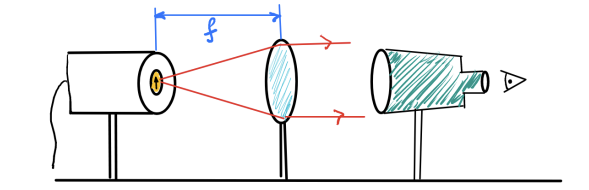
\includegraphics[width=0.5\linewidth]{pics/ust-1.png}
    \caption{}
    \label{fig:ust-1}
\end{figure}

2) Собираем установку с рис. \ref{fig:ust-1}, находя лучшее изображение рисунка на транспаранте, находим следующие значения фокусов линз:

\begin{table}[H]
\centering
	\begin{tabular}{|c|c|c|}
	\hline
	№ линзы & тип линзы & F, см \\ \hline
	3.1 & собирающая & 8.1 \\ \hline
	3.2 & собирающая & 14.9 \\ \hline
	3.3 & собирающая & 20.2 \\ \hline
	3.4 & собирающая & 29.8 \\ \hline
	3.5 & рассеивающая & -10.0 \\ \hline
        3.6 & собирающая & 5.3 \\ \hline    
	\end{tabular}
\end{table}

3) - 4) Чтобы проверить линзы на "тонкость", смотрим на фокусное расстояние развернутых линз:

\begin{table}[H]
\centering
	\begin{tabular}{|c|c|c|}
	\hline
	№ линзы & тип линзы & F, см \\ \hline
	3.1 & собирающая & 7.8 \\ \hline
	3.2 & собирающая & 15.2 \\ \hline
	3.3 & собирающая & 20.3 \\ \hline
	3.4 & собирающая & 30.1 \\ \hline
	3.5 & рассеивающая & -10.0 \\ \hline
        3.6 & собирающая & 5.1 \\ \hline    
	\end{tabular}
\end{table}

В общем, видим что разница укладывается в погрешность что мы оценим чуть позже $\Rightarrow$ все линзы можно с хорошей точностью считать тонкими. 

5) Найдем среднее квадратичное отклоенение $\sigma_F$ по следующим данным: 

\begin{table}[H]
\begin{tabular}{|c|c|c|c|c|c|}
\hline
$n$ & 1    & 2    & 3    & 4    & 5    \\ \hline
$f$, см & 14.8 & 14.7 & 15.1 & 14.8 & 15.5 \\ \hline
\end{tabular}
\end{table}

$\overline{F} = 14.9$ см, $\sigma_F = 0.3$ см, итого измерительная погрешность данного пункта: $\Delta F = 0.1$ см, итоговая $\Delta F = \sqrt{0.3^2 + 0.1^2} \approx 0.3$ см.

\begin{figure}[h]
    \centering
    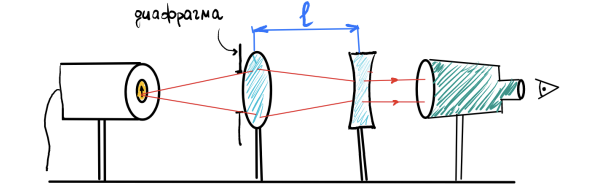
\includegraphics[width=0.5\linewidth]{pics/ust-2.png}
    \caption{}
    \label{fig:ust-2}
\end{figure}

6) Для рассеивающей линзы собираем схему с рис. \ref{fig:ust-2}, для удобства берем линзу 3.1, и ставим ее на расстояние 16 см от транспаранта и получаем четкое изображение в зрительной трубе при расстоянии в 6 см между линзами системы, путем двойного применения ФТЛ, получаем что $F_{\text{расс}} = -10$ см. Погрешность данного измерения: $\Delta F_{\text{расс}} = \Delta d + \Delta l = d^2 \left( \frac{\Delta F}{F^2} + \frac{\Delta f}{f^2}\right) + 0.1 = 0.5 + 0.1 = 0.6$ см

\subsection*{ Измерение фокусных расстояний линз по формуле тонкой линзы и
методом Бесселя}

\begin{figure}[h]
    \centering
    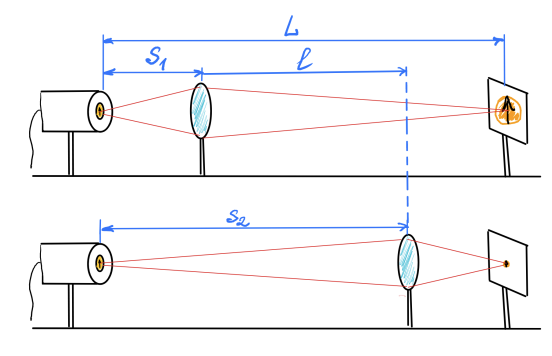
\includegraphics[width=0.5\linewidth]{pics/ust-3.png}
    \caption{}
    \label{fig:ust-3}
\end{figure}

\textbf{1.} Установим линзу 3.1 между экраном и источником. Экран же расположим на расстоянии $L \sim 1,2 \cdot 4F_{3.2}$. $L = (59.5 \pm 0,2)$ см.

\textbf{2.} Перемещая линзу, получим 2 различных действительных изображения - увеличенное и уменьшенное. Измерим для каждого из случаев расстояние от линзы до источника $s_1 = 25.5 \pm 0,2$ см и $s_2 = 35.0 \pm 0,2$ см. $l = s_2 - s_1 = 9.5 \pm 0,4$ см.

\textbf{3.} Теперь по формуле тонкой линзы и по формуле Бесселя найдём фокусное расстояние линзы($f = \frac{L^2 - l^2}{4L}$, и $F_i = \frac{s_i\cdot(L-s_i)}{L}$). Получилось 3 значения фокусного расстояния.
$F_1 = 14.8 \pm 0,5$ см, $F_2 = 14.7 \pm 0,5$ см, $F_\text{Б} = 14.5 \pm 0,3$ см, погрешности оценим из формул из 6) пункта прошлого раздела.

\subsection*{Измерение фокусных расстояний методом Аббе}

\begin{figure}[h]
    \centering
    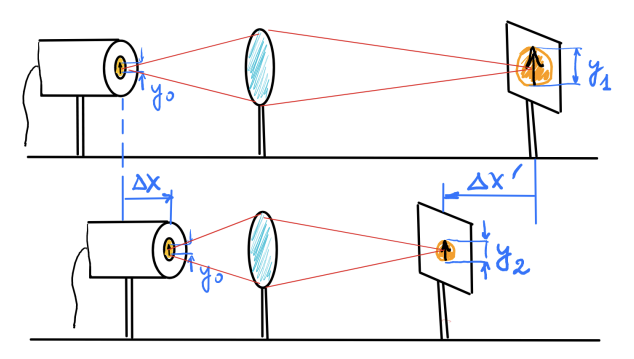
\includegraphics[width=0.5\linewidth]{pics/ust-4.png}
    \caption{}
    \label{fig:ust-4}
\end{figure}

\textbf{1.} Установим линзу 3.1 между экраном и источником. На источнике есть предмет, линейный размер измерим линейкой $y_0 = (1,3 \pm 0,1)$ см. 

\textbf{2.} Перемещая линзу вдоль скамьи, найдём положение действительного изображения на экране и измерим его линейный размер $y_1 =  (3.3 \pm 0,1)$ см.

\textbf{3.} Оставляя линзу в прежнем положении, сдвинем источник на $\Delta x = (4,0 \pm 0,1)$ см. 

\textbf{4.} Теперь сместим нашу линзу так, чтобы вновь получить действительное изображение. Данное смещение равно $\Delta x' = (9.1 \pm 0,1)$ см. Измерим новый линейный размер изображения $y_2 = (2.5 \pm 0,1)$ см.

\textbf{5.} Вычислим значение фокусного расстояния методом Аббе ($f_1 = \frac{\Delta x'}{\frac{y_1}{y_0}-\frac{y_2}{y_0}}, f_2 = \frac{\Delta x}{\frac{y_0}{y_2}-\frac{y_0}{y_1}}$) $f_1 = (14.6 \pm 5.1)$ см $f_2 = (14.9 \pm 6.2)$ см. Погрешность считаем по следующей формуле: $\Delta f_1 = f_1 \left( \frac{\Delta l}{\Delta x} + \frac{\frac{y_1}{y_0} \left(\frac{\Delta l}{y_1} + \frac{\Delta l}{y_0}\right) + \frac{y_2}{y_0} \left( \frac{\Delta l}{y_2} + \frac{\Delta l}{y_0} \right)}{\frac{y_1}{y_0} - \frac{y_2}{y_0}}\right)$, для $f_2$, аналогично.

\subsection*{Сборка и изучение подзорных труб Кеплера}

\begin{figure}[h]
    \centering
    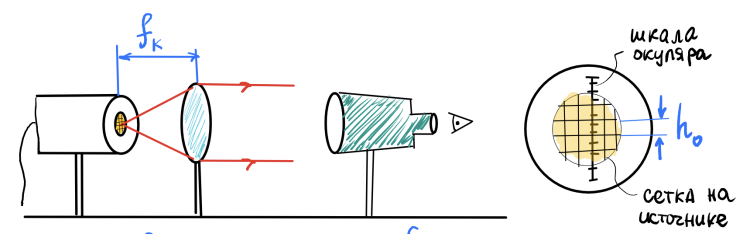
\includegraphics[width=0.5\linewidth]{pics/ust-5.png}
    \caption{}
    \label{fig:ust-5}
\end{figure}

\textbf{1.} Из набора линза выберим три. $F_{3.2}$ - коллиматор, $F_{3.4}$ - объектив, $F_{3.1}$ - окуляр.

\textbf{2.} С помощью подзорной трубы установим коллиматорную линзу перед источником так, чтобы транспарант оказался строго в фокусе линзы. (как на рис. \ref{fig:ust-5})

\textbf{3.} С помощью подзорной трубы оценим сколько ячеек сетки изображения укладывается в поле зрения на размере окулярной риски. Получилось на 1 риску 0.4 сетки.

\begin{figure}[h]
    \centering
    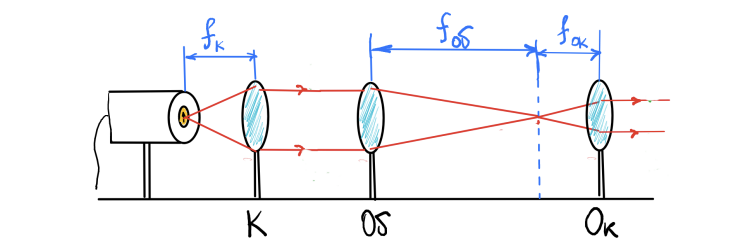
\includegraphics[width=0.5\linewidth]{pics/ust-6.png}
    \caption{}
    \label{fig:ust-6}
\end{figure}
\newpage
\textbf{4.} Соберём на скамье телескоп Кеплера. Для этого собирающую линзу с наибольшим фокусным расстоянием - объектив телескопа - расположим сразу за коллиматором. Вторую же линзу - окуляр телескопа - установим на расстоянии $F_\text{об} + F_\text{ок}$ от объектива (как на рис. \ref{fig:ust-6}). При непосредственном наблюдении глазом будет видно увеличенное изображение сетки на поверхности источника.

\textbf{5.} При установке вспомогательной зрительной трубы, получилось, что на 1 риску приходится 1.6 сетки. Получается $\gamma_\text{эксп} = 4$, а $\gamma_\text{теор} = 3.7$. Такое расхождение может возникнуть из-за недостаточного точного измерения фокусных расстояний линз, а также из-за измерения количество сеток на 1 риску "на глаз".

\textbf{6.} Теперь с помощью тонкого листа бумаги и линейки измерим диаметр $D_\text{об}$ светового пятна, падающего на объектив, и диаметр светового пятна за окуляром $D_\text{ок}$. $D_\text{об} = 3.8$ см, $D_\text{ок} = 1.5$ см. $\gamma = 2.533$, уверен что ошибка вышла из-за обрезания куска светового пучка, на практике это тоже было заметно.

\begin{figure}[h]
    \centering
    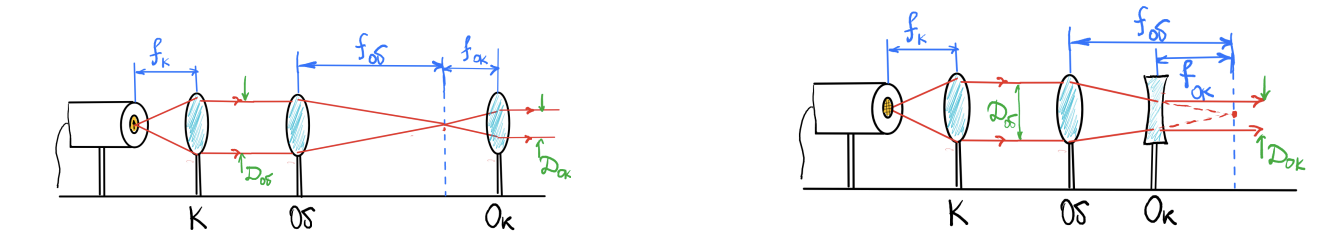
\includegraphics[width=1\linewidth]{pics/ust-7.png}
    \caption{}
    \label{fig:ust-7}
\end{figure}
\newpage
\subsection*{Сборка и изучение модели микроскопа}
\begin{figure}[h]
    \centering
    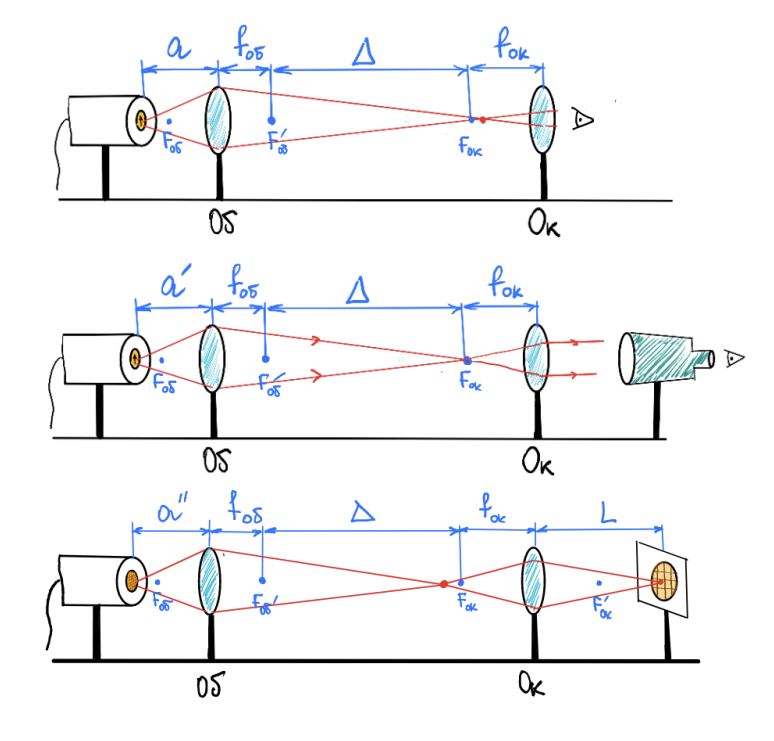
\includegraphics[width=0.55\linewidth]{pics/ust-8.png}
    \caption{}
    \label{fig:ust-8}
\end{figure}
Увеличение микроскопа вычисляется по формуле:
\begin{equation}
    \gamma_M = \Gamma_{o_b} \Gamma_{o_c} = \frac{d}{f_\text{об}} \frac{L}{f_\text{ок}},
\end{equation}
где $f_\text{об}$ и $f_\text{ок}$ - фокусные расстояния линз микроскопа, $d = 23$ см - длина тубуса, $L$ - расстояние наилучшего зрения ($L = 28$ см).\\
Используемые линзы: $F_{3.2} = f_\text{об} = 14.8$ см, $F_{3.1} = f_\text{ок} = 8.1$ см. Получим
    \begin{center}
        $\gamma_{M \text{теор}} = \frac{d}{f_\text{об}} \frac{L}{f_\text{ок}} = 5,37$ \par
        $\gamma_M = \frac{h_2}{h_1}  = (5,23 \pm 0,32)$ \par
        $\Delta \gamma_M = \gamma_M \left( \frac{\Delta h_2}{h_2} + \frac{\Delta h_1}{h_1}\right) = 0.32$
    \end{center}
Видим, что значения практически совпадают.

\subsection*{Изучение составной оптической системы}

1) Берем линзы 3.1 и 3.5, измеряем расстояние между линзами $l = 5$ см, получаем что по формуле для $f$: 
\begin{equation*}
    f = \left( \frac{1}{f_1} + \frac{1}{f_2} - \frac{l}{f_1 \cdot f_2} \right)^{-1} = 16.5 \text{см}
\end{equation*}
Сразу оцениваем что суммарное фокусное расстояние положительное $\Rightarrow$ получаем совпадение с теорией

2) С помощью зрительной трубы измеряем фокусные расстояния с двух сторон от системы, получаем: 
$$F_1 = 14 \text{см}$$
$$F_2 = 17 \text{см}$$
На самом деле, по ощущениям, значения получены с погрешностью в 1-2 сантиметра, потому что получить достаточно четкое изображение не получилось. Как и провести измерения методом Аббе, Бесселя.

\section*{Вывод}
В ходе данной работы были изучены методы определения фокусных расстояний линз. Так, различными способами были как оценены, так и вычислены фокусные расстояния как различных собирающихся линз, так и рассеивающей. Все изученные методы давали значения фокусного расстояние, близкие друг к другу(так, при помощи подзорной трубы $F_{1.1} = 14.8 \pm 0,1$ см, методом Бесселя $F_{3.2} = 14.9 \pm 0,5$ см, методом Аббе $F_{1.1} = 14.6 \pm 5.1$ см. Также была собрана подзорная труба Кеплера, с помощью неё вычислено увеличение телескопа($\gamma = 4$, $\gamma = 2.5$), которое получилось достаточно схожим с полученным теоретически($\gamma = 3.7$), кроме конечно второго, потому что часть светового пучка была обрезана.
\end{document}

\end{document}